\title{Os bastidores da Ciência do Solo}
\author{por Otávio Antonio de Camargo}
\maketitle
\begin{wrapfigure}{l}{0.15\textwidth}
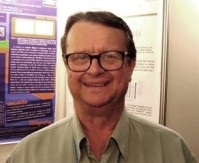
\includegraphics[width=0.15\textwidth]{figuras/foto-otavio-camargo}
\end{wrapfigure}

A qualidade do ambiente interessa a toda a sociedade.  A pureza do ar, da água e do solo é de fundamental importância para a sobrevivência do homem. Em muitas regiões do globo, os índices mínimos de pureza já não são mais alcançados. Muitos rios, lagos e represas tornaram-se depósito de resíduos urbanos, agrícolas e industriais, os solos vêm sendo degradados química, física e biologicamente e o ar tornou-se irrespirável.

A população,  percebeu a ameaça à sua existência e, então, vem reagindo de maneira firme contra a destruição do meio que a cerca, culminando com a ECO-92 e a Agenda 21.

Embora a definição de sustentabilidade seja ainda pouco consensual e às vezes até mesmo contraditória, prejudicando a definição de uma estratégia para um desenvolvimento sustentável, parece-me que, mesmo intuitivamente pensando, é o caminho que temos escolhido nas últimas décadas do 2$^\circ$ milênio.

É assim que me permito uma primeira reflexão apoiada na de Girt e que acho muito oportuna e que fosse embutida e considerada nas discussões onde se fala em desenvolvimento sustentável onde é preciso reconciliar aspectos econômicos e sociais com as dimensões biofísicas referentes aos recursos naturais e à própria capacidade dos distintos ecossistemas em responder à demanda que lhes submetam as sociedades humanas. 

O uso inadequado do solo é fonte muito importante de poluição. O descuido do homem em controlar a erosão, por exemplo, faz do solo uma fonte potencial de contaminação de correntezas e lagos, isso sem contar a sua própria perda.

O manejo inadequado de defensivos, águas de irrigação de baixa qualidade, a disposição indisciplinada de resíduos da agricultura, indústria e cidades podem redundar no acúmulo de substâncias no solo que podem ser tóxicas às plantas e, se entrarem na cadeia alimentar, podem ser letais aos animais e ao homem.

Devido a estas relações e dada sua importância no ecossistema, o solo ocupa papel de destaque no controle da qualidade do ambiente. Se esse controle vai ser de boa ou má qualidade dependerá muito da maneira como serão manejadas as reservas edáficas.

Entretanto, deve-se ter em conta em nossas discussões, mesmo que puramente técnicas, que a degradação destes recursos não é consequência inevitável do progresso humano e mesmo da densidade das populações, mas consequência de um tipo de crescimento econômico cruelmente insustentável em termos ecológicos, e desigual e injusto em termos sociais. É bom que se perceba que a degradação ambiental não é consequência do desenvolvimento, mas de uma modalidade particular deste, fazendo-se assim necessária e urgente uma correção significativa de rota.

A solução não estará então em desacelerar o desenvolvimento, mas mudar qualitativa e quantitativamente o modelo, mantendo como alvo primacial o melhoramento da qualidade de vida, porém nem sempre pensando o crescimento como aumento da produção.

Para tanto não podemos ter um Estado pequeno, fragmentado e frágil, como vemos acontecer em muitas partes do globo atualmente, mas um Estado, se pequeno, sadio e robusto, para evitar a palavra forte. A visível deterioração das instituições  públicas nos últimos anos com a difusão da ideia de enxugamento da máquina como parte do processo de modernização administrativa é um caminho muito negativo se não forem definidas urgentemente as funções que o Estado deve desempenhar na promoção de um desenvolvimento sustentável.

Explico, é consenso que um zoneamento agroecológico e o planejamento do uso da terra são ingredientes primordiais para qualquer definição de estratégia de desenvolvimento sustentável a ser adotada. Portanto, parece-me ter cabimento a pergunta: pode-se esperar sucesso de qualquer modelo nesse sentido diante de um Estado debilitado?

O momento é de muita reflexão e me resta pensar que o homem só conservará sua saúde biológica e mental se aprender a criar um ambiente sadio.

E gostaria de terminar essas poucas e rápidas reflexões com a observação feita pelo escritor Henry Thoreau: ``de que vale uma casa quando não se tem um planeta tolerável onde colocá-la?''

\address{Otávio Antonio de Camargo\\
  Instituto Agronômico de Campinas, IAC\\
  \url{http://lattes.cnpq.br/1337171805613486}\\
  \email{ocamargo@iac.sp.gov.br}}
%%% Local Variables: 
%%% mode: latex
%%% TeX-master: 4th-edition.tex
%%% End: 